\documentclass{article}

\usepackage{amsmath,amsfonts,amsthm,amssymb,amsopn,bm}
\usepackage[margin=.9in]{geometry}
\usepackage{graphicx}
\usepackage{url}
\usepackage[usenames,dvipsnames]{color}
\usepackage{fancyhdr}
\usepackage{listings}
\newcommand{\field}[1]{\mathbb{#1}}
\newcommand{\1}{\mathbf{1}}
\newcommand{\E}{\mathbb{E}} 
\renewcommand{\P}{\mathbb{P}}
\newcommand{\R}{\field{R}} % real domain
% \newcommand{\C}{\field{C}} % complex domain
\newcommand{\F}{\field{F}} % functional domain

\newcommand{\T}{^{\textrm T}} % transpose

\def\diag{\text{diag}}

%% operator in linear algebra, functional analysis
\newcommand{\inner}[2]{#1\cdot #2}
\newcommand{\norm}[1]{\left\|#1\right\|}
\newcommand{\twonorm}[1]{\|#1\|_2^2}
% operator in functios, maps such as M: domain1 --> domain 2
\newcommand{\Map}[1]{\mathcal{#1}}
\renewcommand{\theenumi}{\alph{enumi}} 

\newcommand{\Perp}{\perp \! \! \! \perp}

\newcommand\independent{\protect\mathpalette{\protect\independenT}{\perp}}
\def\independenT#1#2{\mathrel{\rlap{$#1#2$}\mkern2mu{#1#2}}}
\newcommand{\vct}[1]{\boldsymbol{#1}} % vector
\newcommand{\mat}[1]{\boldsymbol{#1}} % matrix
\newcommand{\cst}[1]{\mathsf{#1}} % constant
\newcommand{\ProbOpr}[1]{\mathbb{#1}}
\newcommand{\grade}[1]{\small\textcolor{magenta}{\emph{[#1 points]}} \normalsize}
\date{{}}

\setlength\parindent{0px}

\begin{document}
\title{Homework \#0}
\author{\normalsize{CSE 546: Machine Learning}\\
\normalsize{Michael Ross} \\
\normalsize{Due: 10/4/18  11:59 PM}}
\maketitle


\section{Analysis}

1. \grade{1} A set $A \subseteq \R^n$ is \emph{convex} if $\lambda x + (1-\lambda) y \in A$ for all $x,y\in A$ and $\lambda \in [0,1]$.
A \emph{norm} $\|\cdot\|$ over $\R^n$ is defined by the properties:
i) non-negative: $\|x\|\geq 0$ for all $x \in \R^n$ with equality if and only if $x=0$,
ii) absolute scalability: $\|a \, x\| = |a| \, \|x\|$ for all $a \in \R$ and $x \in \R^n$, iii) triangle inequality: $\|x+y\| \leq \|x\| + \|y\|$ for all $x,y \in \R^n$.
\begin{enumerate}
	\item Using just the definitions above, show that the set $\{ x \in \R^n : \|x\| \leq 1\}$ is convex for any norm $\| \cdot \|$.\\
	\textbf{Answer:} \\
	Let $A=\{ x \in \R^n : \|x\| \leq 1\}$ and $x,y\in A$\\
	\\
	$\norm{\lambda x+(1-\lambda)y}=\norm{\lambda x}+\norm{(1-\lambda)y}=|\lambda|\norm{x}+|1-\lambda|\norm{y}$\\
	$|\lambda|\in[0,1]$ by norm definition\\
	$\norm{x}\in[0,1]$ by norm and set definitions\\
	$\norm{y}\in[0,1]$ by norm and set definitions\\
	$\implies \norm{\lambda x+(1-\lambda)y}\leq1$\\
	\\
	$\lambda x+(1-\lambda)y$ is a linear combination of elements of $\R^n$\\
	$\implies \lambda x+(1-\lambda)y\in \R^n$\\
	\\
	Thus $\lambda x+(1-\lambda)y \in A$ for any $x,y$
	
	\item Show that $\left(\sum_{i=1}^n |x_i|^{1/2}\right)^2$ is or is not a norm.\\
	\textbf{Answer:} \\
	i) $x_i\in \R$\\
	$\implies |x_i|^{1/2}\in\R $\\
	$\implies \sum_{i=1}^n|x_i|^{1/2}\in\R $\\
	$\implies \left(\sum_{i=1}^n |x_i|^{1/2}\right)^2\geq0 $\\
	\\
	ii) $\norm{a x}=\left(\sum_{i=1}^n |a x_i|^{1/2}\right)^2$\\
	$=\left(\sum_{i=1}^n (|a| |x_i|)^{1/2}\right)^2$\\
	$=\left(\sum_{i=1}^n |a|^{1/2} |x_i|^{1/2}\right)^2$\\
	$=\left(|a|^{1/2}\sum_{i=1}^n  |x_i|^{1/2}\right)^2$\\
	$=\left|a|(\sum_{i=1}^n  |x_i|^{1/2}\right)^2$\\
	$=|a|\norm{x}$\\
	\\
	iii)
\end{enumerate} 

2. \grade{1} For any $x \in \R^n$, define the following norms: $\|x\|_1 = \sum_{i=1}^n |x_i|$, $\|x\|_2 = \sqrt{\sum_{i=1}^n |x_i|^2}$, $\|x\|_\infty = \max_{i=1,\dots,n} |x_i|$. Show that $\|x\|_\infty \leq \|x\|_2 \leq \|x\|_1$.\\

3. \grade{1} For possibly non-symmetric $\mat{A}, \mat{B} \in \R^{n \times n}$ and $c \in \R$, let $f(x, y) = x^T \mat{A} x + y^T \mat{B} x + c$. Define $\nabla_z f(x,y) = \begin{bmatrix} \frac{\partial f(x,y)}{\partial z_1} & \frac{\partial f(x,y)}{\partial z_2} & \dots & \frac{\partial f(x,y)}{\partial z_n} \end{bmatrix}^T$.  What is $\nabla_x f(x,y)$ and $\nabla_y f(x,y)$? \\

4. \grade{1} Let $\mat{A}$ and $\mat{B}$ be two $\R^{n\times n}$ symmetric
matrices. Suppose $\mat{A}$ and $\mat{B}$ have the exact same set of eigenvectors
$\vct{u}_1, \vct{u}_2, \cdots, \vct{u}_n$ with the corresponding
eigenvalues $\alpha_1, \alpha_2, \cdots, \alpha_{n}$ for $\mat{A}$, and
$\beta_1, \beta_2, \cdots, \beta_{n}$ for $\mat{B}$. Please write down
the eigenvectors and their corresponding eigenvalues for the following matrices:
\begin{enumerate}
\item $\mat{C} = \mat{A}+\mat{B}$\\
\textbf{Answer:} \\
Eigenvectors: $\mathbf{u_1},\mathbf{u_2},...\mathbf{u_n}$	Eigenvalues: $\alpha_1+\beta_1, \alpha_2+\beta_2,...\alpha_n+\beta_n$
\item $\mat{D} = \mat{A} - \mat{B}$\\
\textbf{Answer:} \\
Eigenvectors: $\mathbf{u_1},\mathbf{u_2},...\mathbf{u_n}$	Eigenvalues: $\alpha_1-\beta_1, \alpha_2-\beta_2,...\alpha_n-\beta_n$
\item $\mat{E} = \mat{A}\mat{B}$\\
\textbf{Answer:} \\
Eigenvectors: $\mathbf{u_1},\mathbf{u_2},...\mathbf{u_n}$	Eigenvalues: $\alpha_1\beta_1, \alpha_2\beta_2,...\alpha_n\beta_n$
\item $\mat{F} = \mat{A}^{-1}\mat{B}$ (\mbox{assume $\mat{A}$ is invertible})\\
\textbf{Answer:} \\
Eigenvectors: $\mathbf{u_1},\mathbf{u_2},...\mathbf{u_n}$	Eigenvalues: $\beta_1/\alpha_1, \beta_2/\alpha_2,...\beta_n/\alpha_n$
\end{enumerate}

5. \grade{1} A symmetric matrix $\mat{A} \in \R^{n \times n}$ is \emph{positive-semidefinite (PSD)} if $x^T \mat{A} x \geq 0$ for all $x \in \R^n$. 
\begin{enumerate} 
	\item For any $y \in \R^n$, show that $y y^T$ is PSD. \\
	\textbf{Answer:} \\
	$x^Tyy^Tx=(x\cdot y)(y\cdot x)=(x\cdot y)^2\geq0$
	\item Let $X$ be a random vector in $\R^n$ with covariance matrix $\mat{\Sigma} =
\ProbOpr{E}[(X-\ProbOpr{E}[X])(X-\ProbOpr{E}[X])\T]$. Show that $\mat{\Sigma}$ is PSD. \\
\textbf{Answer:} \\
$x^T\Sigma x=x^T\ProbOpr{E}[(X-\ProbOpr{E}[X])(X-\ProbOpr{E}[X])\T]x$\\
$=\ProbOpr{E}[x^T(X-\ProbOpr{E}[X])(X-\ProbOpr{E}[X])\T x]$ since x is not random $x\ProbOpr{E}[X]=\ProbOpr{E}[xX]$\\
Let $\gamma=(X-\ProbOpr{E}[X])^T x=x^T (X-\ProbOpr{E}[X])$\\
$x^T\Sigma x=\ProbOpr{E}[\gamma^2]$\\
$\gamma\in\R\implies\gamma^2\geq0\implies\ProbOpr{E}[\gamma^2]\geq0$\\
$\implies x^T\Sigma x\geq0$

	\item Assume $\mat{A}$ is a symmetric matrix so that $\mat{A} = \mat{U} \diag(\alpha) \mat{U}^T$ where $\diag({\alpha})$ is an all zeros matrix with the entries of ${\alpha}$ on the diagonal and $\mat{U}^T \mat{U} = I$. Show that $\mat{A}$ is PSD if and only if $\min_i \alpha_i \geq 0$. (Hint: compute $x^T \mat{A} x$ and consider values of $x$ proportional to the columns of $\mat{U}$, i.e., the orthonormal eigenvectors).\\
\textbf{Answer:} \\
$x^T A x=x^T \mat{U} diag(\alpha) \mat{U}^T x$\\
Let $x=\mat{U}\beta$ where $\beta \in \R^n$\\
$x^T A x=\beta^T \mat{U}^T \mat{U} diag(\alpha) \mat{U}^T \mat{U} \beta$\\
$=\beta^T diag(\alpha) \beta$\\
Switching to index notation\\
$=\beta_i diag(\alpha)_{ij} \beta_j$\\
$diag(\alpha)_{ij}=0$ for $i\neq j$\\
$\implies x^T A x=\sum_{i=1}^n\beta_i\beta_i\alpha_i$
\end{enumerate}

6. \grade{1} Let $X$ and $Y$ be real independent random variables with PDFs given by $f$ and $g$, respectively. Let $h$ be the PDF of the random variable $Z = X+Y$.
\begin{enumerate}
	\item Derive a general expression for $h$ in terms of $f$ and $g$
	\item If $X$ and $Y$ are both independent and uniformly distributed on $[0,1]$ (i.e. $f(x)=g(x)=1$ for $x \in [0,1]$ and $0$ otherwise) what is $h$, the PDF of $Z=X+Y$?
	\item For these given explicit distributions, what is $\P(X \leq 1/2 | X+Y\geq 5/4)$?
\end{enumerate}

7. \grade{1} A random variable $X \sim \mathcal{N}(\mu, \sigma^2)$ is Gaussian distributed with mean $\mu$ and variance $\sigma^2$. Given that for any $a,b \in \R$, we have that $Y = aX + b$ is also Gaussian, find $a,b$ such that $Y \sim \mathcal{N}(0,1)$.\\
\textbf{Answer:}\\
$\ProbOpr{E}[Y]=0$\\
$a \ProbOpr{E}[X]+b=0$\\
$a\mu+b=0$\\
$\mu=-b/a$\\
\\
$\ProbOpr{E}[Y^2]-\ProbOpr{E}[Y]^2=1$\\
Since $\ProbOpr{E}[Y]=0$\\
$\ProbOpr{E}[Y^2]=1$\\
$\ProbOpr{E}[a^2 X^2+2abX+b^2]=1$\\
$a^2 \ProbOpr{E}[X^2]+2ab\ProbOpr{E}[X]+b^2=1$\\
$a^2 \ProbOpr{E}[X^2]-a^2\ProbOpr{E}[X]^2+a^2\ProbOpr{E}[X]^2+2ab\ProbOpr{E}[X]+b^2=1$\\
$a^2 \sigma^2+a^2\mu^2+2ab\mu+b^2=1$\\
Plug $\mu=-b/a$ in\\
$a^2 \sigma^2+b^2-2b^2+b^2=1$\\
$\implies a=1/\sigma$\\
$\implies b=-\mu/\sigma$\\

8. \grade{1} If $f(x)$ is a PDF, we define the cumulative distribution function (CDF) as $F(x) = \int_{-\infty}^x f(y) dy$.
For any function $g : \R \rightarrow \R$ and random variable $X$ with PDF $f(x)$, define the expected value of $g(X)$ as $\E[g(X)] = \int_{-\infty}^\infty g(y) f(y) dy$. For a boolean event $A$, define $\1\{ A \}$ as $1$ if $A$ is true, and $0$ otherwise. Thus, $\1\{ x \leq a \}$ is $1$ whenever $x \leq a$ and $0$ whenever $x > a$. 
Note that $F(x) = \E[\1\{X \leq x\}]$.
Let $X_1,\dots,X_n$ be \emph{independent and identically distributed} random variables with CDF $F(x)$. 
Define $\widehat{F}_n(x) = \frac{1}{n} \sum_{i=1}^n \1\{X_i \leq x\}$.
\begin{enumerate}
	\item For any $x$, what is $\E[ \widehat{F}_n(x) ]$?\\
	\textbf{Answer:}\\
	$\E[ \widehat{F}_n(x) ]=\E[\frac{1}{n}  \sum_{i=1}^n \1 \{X_i\leq x \}]$\\
	$=\frac{1}{n}  \sum_{i=1}^n \E[\1 \{X_i\leq x \}]$\\
	$=\frac{1}{n}  \sum_{i=1}^n F(x)$\\
	$=F(x)$\\
	
	\item For any $x$, show that $\E[ ( \widehat{F}_n(x) - F(x) )^2 ] = \frac{F(x)(1-F(x))}{n}$\\
	\textbf{Answer:}\\
	$\E[ ( \widehat{F}_n(x) - F(x) )^2 ]=\E[  \widehat{F}_n(x)^2 -2\widehat{F}_n(x) F(x)+ F(x)^2 ]  $\\
	$=\E[  \widehat{F}_n(x)^2] -2\E[\widehat{F}_n(x)] F(x)+ F(x)^2 ] $\\
	
	 $\widehat{F}_n(x)^2=\frac{1}{n^2}(\sum_{i=1}^n \1\{X_i \leq x\})^2$\\
	 $=\frac{1}{n^2}(\sum_{i=1}^n \1\{X_i \leq x\}\1\{X_1 \leq x\}+...+\sum_{i=1}^n \1\{X_i \leq x\}\1\{X_n \leq x\})$\\
	 $=\frac{1}{n^2}(\sum_{i=1}^n \1\{X_i \leq x\}+...+\sum_{i=1}^n \1\{X_i \leq x\})$\\
	 $=\frac{1}{n}\sum_{i=1}^n \1\{X_i \leq x\}$\\
	 $=\widehat{F}_n(x)$
	 
	 $\E[ ( \widehat{F}_n(x) - F(x) )^2 ]=F(x)-2F(x)F(x)+F(x)^2$\\
	 $=F(x)(1-F(x))$\\
	
	\item Using part b., show that $\displaystyle\sup_{x \in \R} \E[ ( \widehat{F}_n(x) - F(x) )^2 ] \leq \tfrac{1}{4n}$. \\
	\textbf{Answer:}\\
	$\displaystyle\sup_{x \in \R} \E[ ( \widehat{F}_n(x) - F(x) )^2 ] =\displaystyle\sup_{x \in \R} \frac{1}{n} (F(x)-F(x)^2)$\\
	
	$\partial_{F(x)} (\frac{1}{n} (F(x)-F(x)^2))=\frac{1}{n} (1-2F(x))$\\
	$\underset{F(x)}{\operatorname{arg\ max}} (\frac{1}{n} (F(x)-F(x)^2))=1/2$\\
	max $(\frac{1}{n} (F(x)-F(x)^2))=\frac{1}{4n}$\\
	$\implies \displaystyle\sup_{x \in \R} \E[ ( \widehat{F}_n(x) - F(x) )^2 ] \leq \frac{1}{4n}$\\
	
\end{enumerate}

\section{Programming}

9. \grade{2} Two random variables $X$ and $Y$ have equal distributions if their CDFs, $F_X$ and $F_Y$, respectively, are equal: $\sup_{x} |F_X(x) - F_Y(x)| = 0$. 
The central limit theorem says that the sum of $k$ independent, zero-mean, variance-$1/k$ random variables converges to a Gaussian distribution as $k$ goes off to infinity.  
We will study this phenomenon empirically (you will use the Python packages Numpy and Matplotlib). 
Define $Y^{(k)} = \frac{1}{\sqrt{k}} \sum_{i=1}^k B_i$ where each $B_i$ is equal to $-1$ and $1$ with equal probability.
It is easy to verify (you should) that $\frac{1}{\sqrt{k}} B_i$ is zero-mean and has variance $1/k$.
\begin{enumerate}
	\item For $i=1,\dots,n$ let $Z_i \sim \mathcal{N}(0,1)$. If $F(x)$ is the true CDF from which each $Z_i$ is drawn (i.e., Gaussian) and $\widehat{F}_n(x) = \frac{1}{n} \sum_{i=1}^n \1\{ Z_i \leq x)$, use the homework problem above to choose $n$ large enough such that $\sup_x \sqrt{\E[ (\widehat{F}_n(x)-F(x))^2 ]} \leq 0.0025$, and plot $\widehat{F}_n(x)$ from $-3$ to $3$. (Hint: use \texttt{Z=numpy.random.randn(n)} to generate the random variables, and \texttt{import matplotlib.pyplot as plt};\\ \texttt{plt.step(sorted(Z), np.arange(1,n+1)/float(n))} to plot).\\
	\textbf{Answer:}
	\begin{lstlisting}[language=Python]
	import matplotlib.pyplot as plt
	import numpy as np
	
	supMax=0.0025
	n=int(1.0/(2.0*supMax)**2)
	Z=np.random.randn(n)
	
	plt.step(sorted(Z),np.arange(1,n+1)/float(n))
	plt.xlabel("Observations")
	plt.ylabel("Probability")
	plt.xlim((-3,3))
	plt.ylim((0,1))
	plt.grid()
	plt.show()

	\end{lstlisting}
	\item For each $k \in \{1, 8, 64, 512\}$ generate $n$ independent copies $Y^{(k)}$ and plot their empirical CDF on the same plot as part a. (Hint: you can use $\texttt{np.sum(np.sign(np.random.randn(n, k))*np.sqrt(1./k), axis=1)}$ to generate $n$ of the $Y^{(k)}$ random variables.)\\
	\textbf{Answer:}
	\begin{lstlisting}[language=Python]
	import matplotlib.pyplot as plt
	import numpy as np

	supMax=0.0025
		n=int(1.0/(2.0*supMax)**2)
	Z=np.random.randn(n)

	k=[1,8,64,512]
	i=1000
	for j in range(len(k)):
		x=np.sum(np.sign(np.random.randn(i, k[j]))*np.sqrt(1./k[j]), axis=1)
		plt.step(sorted(x),np.arange(1,i+1)/float(i))
	
	plt.step(sorted(Z),np.arange(1,n+1)/float(n))
	plt.xlabel("Observations")
	plt.ylabel("Probability")
	plt.xlim((-3,3))
	plt.ylim((0,1))
	k.append('Gaussian')
	plt.legend(k)
	plt.grid()
	plt.show()

\end{lstlisting}
\end{enumerate}
Be sure to always label your axes. 
Your plot should look something like the following (Tip: checkout \texttt{seaborn} for instantly better looking plots.)
\begin{center}
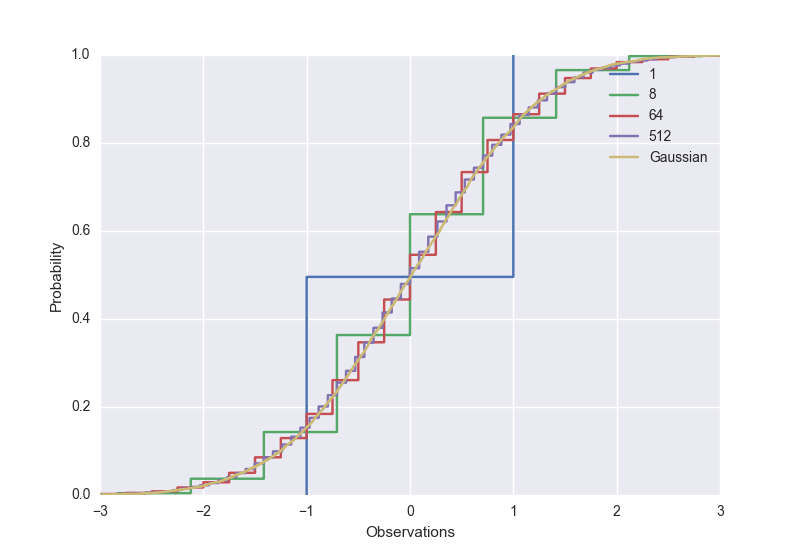
\includegraphics[width=4in]{full.png}
\end{center} 

\end{document}
